%Ще започнем текущата глава от малко по-назад или по-конкретно: ще разгледаме как компютрите са просто детерминирани автомати и как можем да ги обобщим.
\vspace{-0.5cm}
\section{Компютърът - един голям автомат}
\vspace{-0.2cm}
Въпреки, че компютрите обикновено се отъждествяват с детерминирани машини на Тюринг (полезно и от теоретична и от практична гледни точки), те в действителност са детерминирани крайни автомати (тъй като имаме ограничена памет). Нека разгледаме пример.\newline

\begin{examplecp}
	Дадени са следните програми (без вход от потребителя):
	\begin{pseudocode}
		\SetKwData{da}{a}
		
		$Func7():$
		\Mybegin
		{	
			$\da\leftarrow7$\;
			\While{$\da>1$}
			{
				$\da\leftarrow\da-2$\;
			}
			\KwRet{$\da=0$\;}
		}
	\end{pseudocode}
	\begin{pseudocode}
		\SetKwData{da}{a}
		
		$Func4():$
		\Mybegin
		{	
			$\da\leftarrow4$\;
			\While{$\da>1$}
			{
				$\da\leftarrow\da-2$\;
			}
			\KwRet{$\da=0$\;}
		}
	\end{pseudocode}
	\noindent
	Ясно е, че програмите връщат истина т.с.т.к. $a$ е четно и лъжа иначе. Състоянията на автоматите ще бъдат наредени двойки от ред (на програмата) и стойността на променливите (в случая само $a$):
	\begin{itemize}
		\item $a=7$
		\begin{figure}[H]
			\centering
			\scalebox{0.8}{\begin{tikzpicture}[node distance=2cm]				
					\node (17) [state] {$\langle2,?\rangle$};
					\node (27) [state, right of=17] {$\langle3,7\rangle$};
					\node (37) [state, right of=27] {$\langle4,7\rangle$};
					\node (25) [state, right of=37] {$\langle3,5\rangle$};
					\node (35) [state, right of=25] {$\langle4,5\rangle$};
					\node (23) [state, right of=35] {$\langle3,3\rangle$};
					\node (33) [state, right of=23] {$\langle4,3\rangle$};
					\node (21) [state, right of=33] {$\langle3,1\rangle$};
					\node (41) [state, right of=21] {$\langle5,1\rangle$};
					\node (N) [state, right of=41, minimum size=1.4cm] {N};
					
					\draw[arrow] (-1.2,0) -- (17);\draw[arrow] (17) -- (27);
					\draw[arrow] (27) -- (37);\draw[arrow] (37) -- (25);
					\draw[arrow] (25) -- (35);\draw[arrow] (35) -- (23);
					\draw[arrow] (23) -- (33);\draw[arrow] (33) -- (21);
					\draw[arrow] (21) -- (41);\draw[arrow] (41) -- (N);
			\end{tikzpicture}}
		\end{figure}
		
		\item $a=4$
		\begin{figure}[H]
			\centering
			\scalebox{0.8}{\begin{tikzpicture}[node distance=2cm]				
					\node (14) [state] {$\langle2,?\rangle$};
					\node (24) [state, right of=14] {$\langle3,4\rangle$};
					\node (34) [state, right of=24] {$\langle4,4\rangle$};
					\node (22) [state, right of=34] {$\langle3,2\rangle$};
					\node (32) [state, right of=22] {$\langle4,2\rangle$};
					\node (20) [state, right of=32] {$\langle3,0\rangle$};
					\node (40) [state, right of=20] {$\langle5,0\rangle$};
					
					
					\node (Y) [state-final, right of=40, minimum size=1.4cm] {Y};
					
					\draw[arrow] (-1.2,0) -- (14);\draw[arrow] (14) -- (24);
					\draw[arrow] (24) -- (34);\draw[arrow] (34) -- (22);
					\draw[arrow] (22) -- (32);\draw[arrow] (32) -- (20);
					\draw[arrow] (20) -- (40);\draw[arrow] (40) -- (Y);
					
			\end{tikzpicture}}
		\end{figure}
	\end{itemize}
	\noindent
	Макар по дефиниция, ДКА нямат $\varepsilon$-преходи, може да разглеждаме преходите като $\varepsilon$, тъй като от всяко състояние има най-много едно изходно ребро. Разбира се, изложеният метод работи само за предварително фиксирани променливи, т.е. без вход от потребителя. Помислете как бихме могли да обобщим да работи и с вход от потребитля.
\end{examplecp}%\newpage

\section{Недетерминирани алгоритми}

Както вече показахме в предходната секция, всяка програма \textbf{за компютър} може да се представи чрез краен детерминиран автомат. Нека сега да си мислим, че имаме магически компютър, който може да прави много изпълнения едновременно. Лесно се вижда, че такъв магически компютър би се представял чрез краен недетерминиран автомат. Програмите за стандартните компютри описвахме чрез псевдокод. Пргорамите за магическите компютри ще описаваме отново чрез псевдокод, но ще имаме бонус операция - недетерминиран избор. Разбираме се недетерминираните програми/алгоритми да връщат стойности единствено от $\{$TRUE, FALSE$\}$. Аналогично на ДКА, където дума се разпознава, ако има поне едно успешно изпълнение, тук ще връщаме TRUE, ако има поне едно успешно изпълнение.

\begin{boxdefinition}{Изход на недетерминиран алгоритъм}{}
	Ще казваме, че недетерминиран алгоритъм връща TRUE, т.с.т.к. има поне едно успешно изпълнение.
\end{boxdefinition}

\vspace{0.3cm}\noindent
Нека да разледаме слената задача:
\begin{boxzzr}{COMPOSITES}{composites}
	\dproblem{n\in\mathbb{N}^+}{n\text{ съставно ли е?}}
\end{boxzzr}
\begin{solution}
	Ще покажем детерминирано и недетерминирано решение. Да започнем от детерминираното:
	\begin{pseudocode}
		\SetKwData{dn}{n}
		\SetKwData{dq}{q}
		
		$isCompositeDet(\dn)://\,\dn\in\mathbb{N}^+$
		\Mybegin
		{	
			\Myfor{$\dq\leftarrow2$ \KwTo $\lfloor\sqrt{n}\rfloor$}
			{
				\If{$\dn\equiv0\ (\text{mod}\ q)$}{\KwRet{\True\;}}
			}
			
			\KwRet{\False\;}
		}
	\end{pseudocode}
	Коректност няма да разглеждаме. Ясно как става - чрез инвариант. Времевата сложност на тази програма е $O(\sqrt n)$. Големината на входа е $m=\log_2{n}$, т.е. времевата сложност спрямо големината на входа е $O(\sqrt{2^m})=O\big((\sqrt2)^m\big)$ - експоненциална. А дали има полиномиален (спрямо големината на входа) детерминиран алгоритъм?
	
	\vspace{0.3cm}\noindent
	Нека сега разгледаме недетерминиран алгоритъм, решаващ задачата за полиномиално време:
	\begin{pseudocode}
		\SetKwData{dn}{n}
		\SetKwData{dq}{q}
		
		$isCompositeNonDet(\dn)://\,\dn\in\mathbb{N}^+$
		\Mybegin
		{	
			$\dq\leftarrow\Choose(\{2,3,\dots,\lfloor\sqrt n\rfloor\})$\tcp*{недетерминиран избор}
			\If{$\dn\equiv0\ (\text{mod}\ q)$}{\KwRet{\Success\;}}
			
			\KwRet{\Fail\;}
		}
	\end{pseudocode}
	\begin{remark*}
		Можем да правим недетерминиран избор до предварително избрана константа за константно време. В случая, изборът \textbf{НЕ} е ограничен. Това което се случва отдолу е, че всяко битче на числото се избира да е нула или единица.. тоест недетерминираният избор отнема $\Theta(\log_2{\sqrt n})$ време.
	\end{remark*}
	За да докажем коректността на недетерминирания алгоритъм трябва да покажем, че:
	\begin{itemize}
		\item при съставно $n$: има поне едно успешно изпълнение
		\item при просто $n$: всички изпълнения са неуспешни
	\end{itemize}
	Нека $n$ е съставно. Тогава $\big(\exists q_0\in\{2,3,\dots,\lfloor\sqrt n\rfloor\}\big)\big(n\equiv 0\ (\text{mod}\ q_0)\big)$. Ясно е, че клона на изпълнение, в който choose е избрал $q_0$, е успешен. Нека сега $n$ е просто. Тогава знаем, че $\big(\forall q\in\{2,3,\dots,\lfloor\sqrt n\rfloor\}\big)\big(n\not\equiv 0\ (\text{mod}\ q_0)\big)$. Оттук е ясно, че всички изпълнения са неуспешни. Времевата сложност на тази програма е $\Theta(\log_2{\sqrt n})$. Големината на входа е $m=\log_2{n}$, т.е. времевата сложност спрямо големината на входа е $\Theta(\log_2{\sqrt{2^m}})=\Theta(\frac12\log_2(2^m))=\Theta(\frac m2)=\Theta(m)$ - полиномиална.
\end{solution}

\leavevmode\newline\noindent
Нека сега разгледаме допълнението на горната задача и по-конкретно:
\begin{boxzzr}{PRIMES}{primes}
	\dproblem{n\in\mathbb{N}^+}{n\text{ просто ли е?}}
\end{boxzzr}
\begin{solution}
	На пръв поглед, наивното разсъждение \emph{просто ще върнем отрицанието на резултата от COMPOSITES}, ни върши работа. Нека обаче разгледа по-детайлно:
	\begin{pseudocode}
		\SetKwData{dn}{n}
		
		$isPrimeDetNaive(\dn)://\,\dn\in\mathbb{N}^+$
		\Mybegin
		{	
			\KwRet{$\lnot isCompositeDet(\dn)$\;}
		}
	\end{pseudocode}
	Ясно е, че това решение работи. Също така е ясно, че сложността по време е експоненциална.
	
	\vspace{0.3cm}\noindent
	Нека сега разгледаме наивното за недетерминирания алгоритъм:
	\begin{pseudocode}
		\SetKwData{dn}{n}
		
		$isPrimeNonDetNaive(\dn)://\,\dn\in\mathbb{N}^+$
		\Mybegin
		{	
			\KwRet{$\lnot isCompositeNonDet(\dn)$\;}
		}
	\end{pseudocode}
	За да докажем коректността на недетерминирания алгоритъм трябва да покажем, че:
	\begin{itemize}
		\item при просто $n$: има поне едно успешно изпълнение
		\item при съставно $n$: всички изпълнения са неуспешни
	\end{itemize}
	Ще покажем, че второто изискване не е изпълнено. Наистина, нека $n=16$. Клона на изпълнение, в който $choose(\{2,3,4\})$ ни е избрало 3 е успешен, а ние искахме да е неуспешен. Тоест алгоритъмът не е коректен. Не е тривиално да се измисли полиномиален недетерминиран алгоритъм за тази задача.
\end{solution}
\vspace{0.3cm}
\begin{boxremark*}{}
	Нека $\mathscr{A}$ е задача за разпознаване. Тогава
	\begin{itemize}
		\item Ако имаме детерминиран алгоритъм за $\mathscr{A}$, то тривиално получаваме детерминиран алгоритъм за $\overline{\mathscr{A}}$ със същата времева сложност
		\item Ако имаме недетерминиран алгоритъм за $\mathscr{A}$, то нямаме обща схема по която да получим недетерминиран алгоритъм за $\overline{\mathscr{A}}$
	\end{itemize}
\end{boxremark*}

\section{Сводимост и NP-пълнота}

Ще започнем с няколко прости дефиниции. Горе вече споменахме задачи за разпознаване, но не бяхме дали формална дефиниция. За целта нека припомним дефиниция от лекции:

\begin{boxdefinition}{Изчислителна задача}{}
	Изчислителна задача $\mathcal{P}$ ще наричаме двуместна релация $\mathcal{P}\subseteq\mathcal{I}\times\mathcal{S}$, където $\mathcal{I}$ е безкрайно, изброимо множество от екземпляри (instances), а $\mathcal{S}$ е множество от решения (solutions).
\end{boxdefinition}
\begin{boxdefinition}{Задача за разпознаване}{}
	Задача за разпознване $\mathcal{P}$ ще наричаме изчислителна задача $\mathcal{P}\subseteq\mathcal{I}\times\{$TRUE, FALSE$\}$.
\end{boxdefinition}
\noindent
Нека въведем за улеснение следната локална дефиниция:
\begin{boxlocaldefinition*}{}{}
	Ще означаваме с $\mathcal{DP}$ класът от всички задачи за разпознаване.
\end{boxlocaldefinition*}
\noindent
Вече пристъпваме към по-съществените дефиниции от текущата глава:
\begin{boxdefinition}{Класът P}{}
	P $\leftrightharpoons\{\mathcal{P}\in\mathcal{DP}|\big(\doubleexists\mathscr{A}$ - дет. алгоритъм$\big)\big((\mathscr{A}$ \emph{решава положителната част на} $\mathcal{P})\ \&\ (\mathscr{A}$ \emph{има полиномиална времева сложност при изход "да"}$)\big)\}$.
\end{boxdefinition}
\begin{boxdefinition}{Класът NP}{}
	NP $\leftrightharpoons\{\mathcal{P}\in\mathcal{DP}|\big(\doubleexists\mathscr{A}$ - недет. алгоритъм$\big)\big((\mathscr{A}$ \emph{решава положителната част на} $\mathcal{P})\ \&\ (\mathscr{A}$ \emph{има полиномиална времева сложност при изход "да"}$)\big)\}$.
\end{boxdefinition}
\begin{remark*}
	Какво значи алгоритъм да решава изчислителна задача няма да дефинираме формално. В горните две дефиниции се интересуваме само от положителната част на задачата за разпознаване. За отрицателната част нямаме никакви изисквания - алгоритъмът може да връща некоректен резултат, а може даже да зацикля!
\end{remark*}
\noindent
Следните две дефиниции са еквивалентни, но често непрактични:

\begin{boxalternativedefinition*}{Класът P}{}
	P $\leftrightharpoons\{\mathcal{P}\in\mathcal{DP}|\big(\doubleexists\mathscr{A}$ - дет. алг.$\big)\big((\mathscr{A}$ \emph{решава} $\mathcal{P})\ \&\ (\mathscr{A}$ \emph{има полином. вр. сложност}$)\big)\}$.
\end{boxalternativedefinition*}
\begin{boxalternativedefinition*}{Класът NP}{}
	NP $\leftrightharpoons\{\mathcal{P}\in\mathcal{DP}|\big(\doubleexists\mathscr{A}$ - недет. алг.$\big)\big((\mathscr{A}$ \emph{решава} $\mathcal{P})\ \&\ (\mathscr{A}$ \emph{има полином. вр. сложност}$)\big)\}$.
\end{boxalternativedefinition*}
\begin{remark*}
	Употребата на символът $\,\doubleexists\,$ буквално се замества със "съществува". Скобите и логическото изложение са с цел по-лесно възприемане. Аналогично символът $\,\doubleforall\,$ буквално се замества със "за всяко".
\end{remark*}
\noindent
Целта на текущата секция е да даде основи, с които читателят да доказва, че съставянето на полиномиален алгоритъм за даденa ЗЗР е напълно нетривиална задача. За целта, въвеждаме следните две дефиниции:
\begin{boxdefinition}{m-сводимост}{}
	Нека $\mathcal{A},\mathcal{B}\in\mathcal{DP}$. Ще казваме, че $\mathcal{A}$ е m-сводима към $\mathcal{B}$, т.с.т.к. има \textbf{тотална} функция $f$: за всеки екземпляр $x$ на $\mathcal{A}$ е изпълнено:
	\begin{itemize}
		\item $f(x)$ е екземпляр за $\mathcal{B}$
		\item решенията на $\mathcal{A}$ и $\mathcal{B}$ за екземпляри съответно $x$ и $f(x)$ съвпадат
		\item $f$ се изчислява чрез (детерминиран) алгоритъм
	\end{itemize}
	Ще пишем $\mathcal{A}\le_m\mathcal{B}$.
\end{boxdefinition}
\begin{boxdefinition}{Karp\,-\,сводимост (полиномиална m-сводимост)}{}
	Нека $\mathcal{A},\mathcal{B}\in\mathcal{DP}$. Ще казваме, че $\mathcal{A}$ е Karp\,-\,сводима към $\mathcal{B}$, т.с.т.к. има \textbf{тотална} функция $f$: за всеки екземпляр $x$ на $\mathcal{A}$ е изпълнено:
	\begin{itemize}
		\item $f(x)$ е екземпляр за $\mathcal{B}$
		\item решенията на $\mathcal{A}$ и $\mathcal{B}$ за екземпляри съответно $x$ и $f(x)$ съвпадат
		\item $f$ се изчислява чрез детерминиран алгоритъм за полиномиално време
	\end{itemize}
	Ще пишем $\mathcal{A}\le_m^p\mathcal{B}$ или $\mathcal{A}\le_p\mathcal{B}$.
\end{boxdefinition}
\noindent
Вече сме готови да въведем основните (по-интересни) дефиниции:
\begin{boxdefinition}{Класът NP-hard}{}
	NP-h $\leftrightharpoons\{\mathcal{A}\in\mathcal{DP}|\big(\forall\mathcal{B}\in$ NP$\big)\big(\mathcal{B}\le_p\mathcal{A}\big)\}$.
\end{boxdefinition}
\begin{boxdefinition}{Класът NP-complete}{}
	NP-c $\leftrightharpoons$ NP $\cap$ NP-h.
\end{boxdefinition}
\begin{figure}[H]
	\centering
	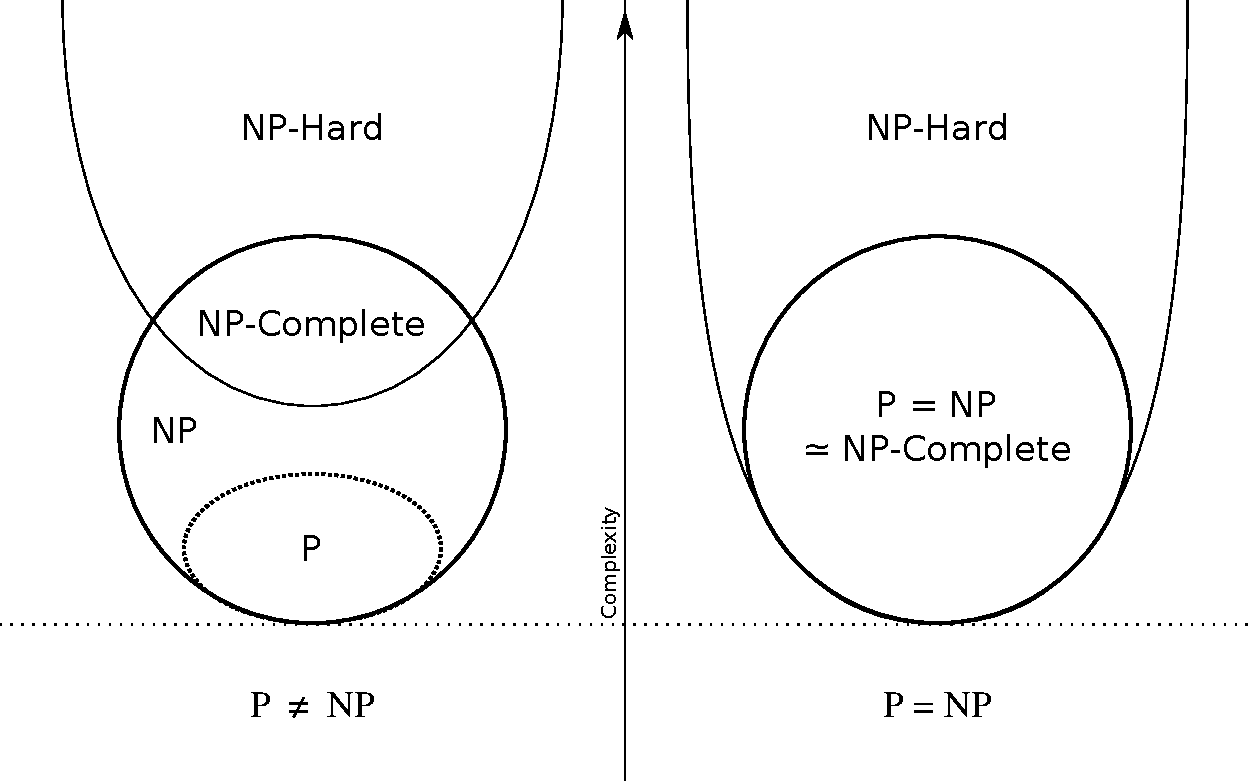
\includegraphics[scale=.4]{images/Euler-Diagram-P-NP-NPh-NPc.pdf}
	\caption{Ойлерова диаграма за класовете P, NP, NP-h и NP-c}
\end{figure}
\noindent
Изобщо не е тривиално да се докаже, че ВСИЧКИ задачи за разпознаване от NP са Karp\,-\,сводими до дадена задача за разпознаване. Ако имаме такава задача и при това намерим детерминирано полиномиално нейно решение, то ще имаме детерминирано полиномиално решение на ВСИЧКИ задачи за разпознаване от NP, откъдето ще следва, че P=NP. Първата задача за разпознаване, за която е доказано, че е NP-hard е така наречената SAT (от satisfiability):
\begin{boxzzr}{SAT}{sat}
	\dproblem{\varphi$ - булева формула в КНФ$}{$Удволетворима ли е $\varphi$?$}
\end{boxzzr}
\begin{examplecp}
	$\begin{cases}
		\varphi=(x_1\lor x_2\lor x_3\lor x_4)\land(\overline{x_1}\lor x_2\lor\overline{x_5}\lor x_8)\land(\overline{x_1}\lor\overline{x_2})\land x_6\land x_7\\\
		\!\!\text{да //сертификат: }\langle x_1,x_2,x_3,x_4,x_5,x_6,x_7,x_8\rangle=\langle T,F,F,T,F,T,T,F\rangle
	\end{cases}$
\end{examplecp}\leavevmode\newline

\begin{boxtheorem}{Cook-Levin}{}
	SAT е NP-трудна.
\end{boxtheorem}
\begin{proof}
	Накратко, само идеята. Всеки недетерминиран алгоритъм може да се представи чрез недетерминирана машина на тюринг (всъщност "истинската"\ дефиницията на NP използва недетерминирани МТ, вместо недетерминирани алгоритми). Тази машина бива представяна чрез булеви формули, т.е. състоянията ѝ, преходите ѝ, началните ѝ състояния, финалните ѝ състояния, лентата ѝ и т.н., като "връзките"\ между тях биват правени отново чрез булеви формули. Съответно тези формули са в КНФ.
\end{proof}\vspace{0.3cm}

\noindent
Следното твърдение ще ни е основният инструмент, с помощта на който ще доказваме, че дадена задача за разпознаване е NP-трудна. Съответно е инструмент, с който да доказваме, че не сме ние глупавите, а че самите задачи са с трудна природа (тоест никой човек досега не е успял да ги реши полиномиално).
\begin{boxproposition}{}{}
	Нека $\mathcal{A},\mathcal{B}\in\mathcal{DP}$. Тогава ако $\mathcal{B}\in$ NP-h и $\mathcal{B}\le_p\mathcal{A}$, то $\mathcal{A}\in$ NP-h.
\end{boxproposition}
\begin{proof}
	Нека $\mathcal{C}$ е произволна от NP. Тъй като $\mathcal{B}\in$ NP-h, то $\mathcal{C}\le_p\mathcal{B}$, но по условие имаме $\mathcal{B}\le_p\mathcal{A}$. Сега от транзитивността имаме $\mathcal{C}\le_p\mathcal{A}$. Но $\mathcal{C}\in$ NP беше произолно, следователно $\big(\forall\mathcal{C}\in$ NP$\big)\big(\mathcal{C}\le_p\mathcal{A}\big)$, т.е. $\mathcal{A}\in$ NP-h (по дефиниция).
\end{proof}